\chapter{Results}
\label{chap:results}

In this section, the results from the proposed solution is described in detail. It describes different results from the different stages throughout the develop process and presents the final results and metrics from the trained \acrfull{ml} model.

\section{Constructed dataset and ML problem formulation}

The initial dataset was copied and validated from \acrfull{mo}'s \acrshort{ais} database. The database table \textit{``vessel\_positions\_history''} was last updated in March 2021 and consists of \textbf{1.2} billion positional \acrshort{ais} records. Each vessel that transmitted positions belongs to a given segment and sub-segment that was made available by the \textit{``vessel\_segment''} table which contains \textbf{eight} different segment values, and \textbf{107} different combinations of segments and sub-segments. The provided \textit{``ports''} data contains \textbf{5200} ports world-wide that all follows the \gls{locode} naming standard. In total, as of March 2021, there were \textbf{6.4} million vessel transitions in the \textit{``vessel\_transitions''} table which was used to construct voyages. This data formed the initial data foundation for the final processed \acrfull{ml} training dataset. All the data that was copied and processed from \acrshort{mo}'s databases were processed in batches. Ports, segments, and transitions where quickly copied and processed, however, the \textbf{1.2} billion positional records took several days to migrate and validate. This was mostly because of the time required to validate coordinates and correctly map \acrshort{mmsi} and \acrshort{imo} values. Throughout this process, the latest identifiers and timestamps were fetched from the dedicated project database to only update data that occurred after the latest records already processed. In this way, this process was idempotent so that running the process multiple times did not affect existing data. This made the system simple to update throughout the development process and as many records as possible were used in the final approach only limited by the thesis time limitation.

\subsection{Voyage definition and construction}

Based on the initial \textbf{6.4} million vessel transitions, \textbf{1.7} million voyages where initially constructed by finding positional records transmitted from a vessel between subsequent departure and arrival transitions. The resulting voyages were, therefore, defined based on transitioning \acrshort{ais} statuses that indicate the vessel is moored or moving. As a consequence of this definition, the quality of the resulting trajectories are very much affected by how well the \gls{aivdm} protocol is followed by the traveling vessels. Since the navigational status attribute is manually inputted by the vessel's captain or crew, the resulting trajectories are prone to human error but results in more complete voyages disregarding intermediate stops for purposes such as bunkering.

As an example, \cref{fig:transition_voyage} shows a voyage from China to Argentina where the vessel stopped at Singapore, most likely to bunker. In the choses voyage definition, the beginning and end of the voyage is defined based on input from the vessel's captain which results in a voyage starting from China, and ending in Argentina. Using an alternative method based on clustering (\cref{sec:vessel_voyage_definition}), this voyage would have been divided into two voyages; one from China to Singapore, and one from Singapore to Argentina. Further advantages and disadvantages is later discussed in \cref{chap:discussion}.

\begin{figure}[htbp]
    \centering
    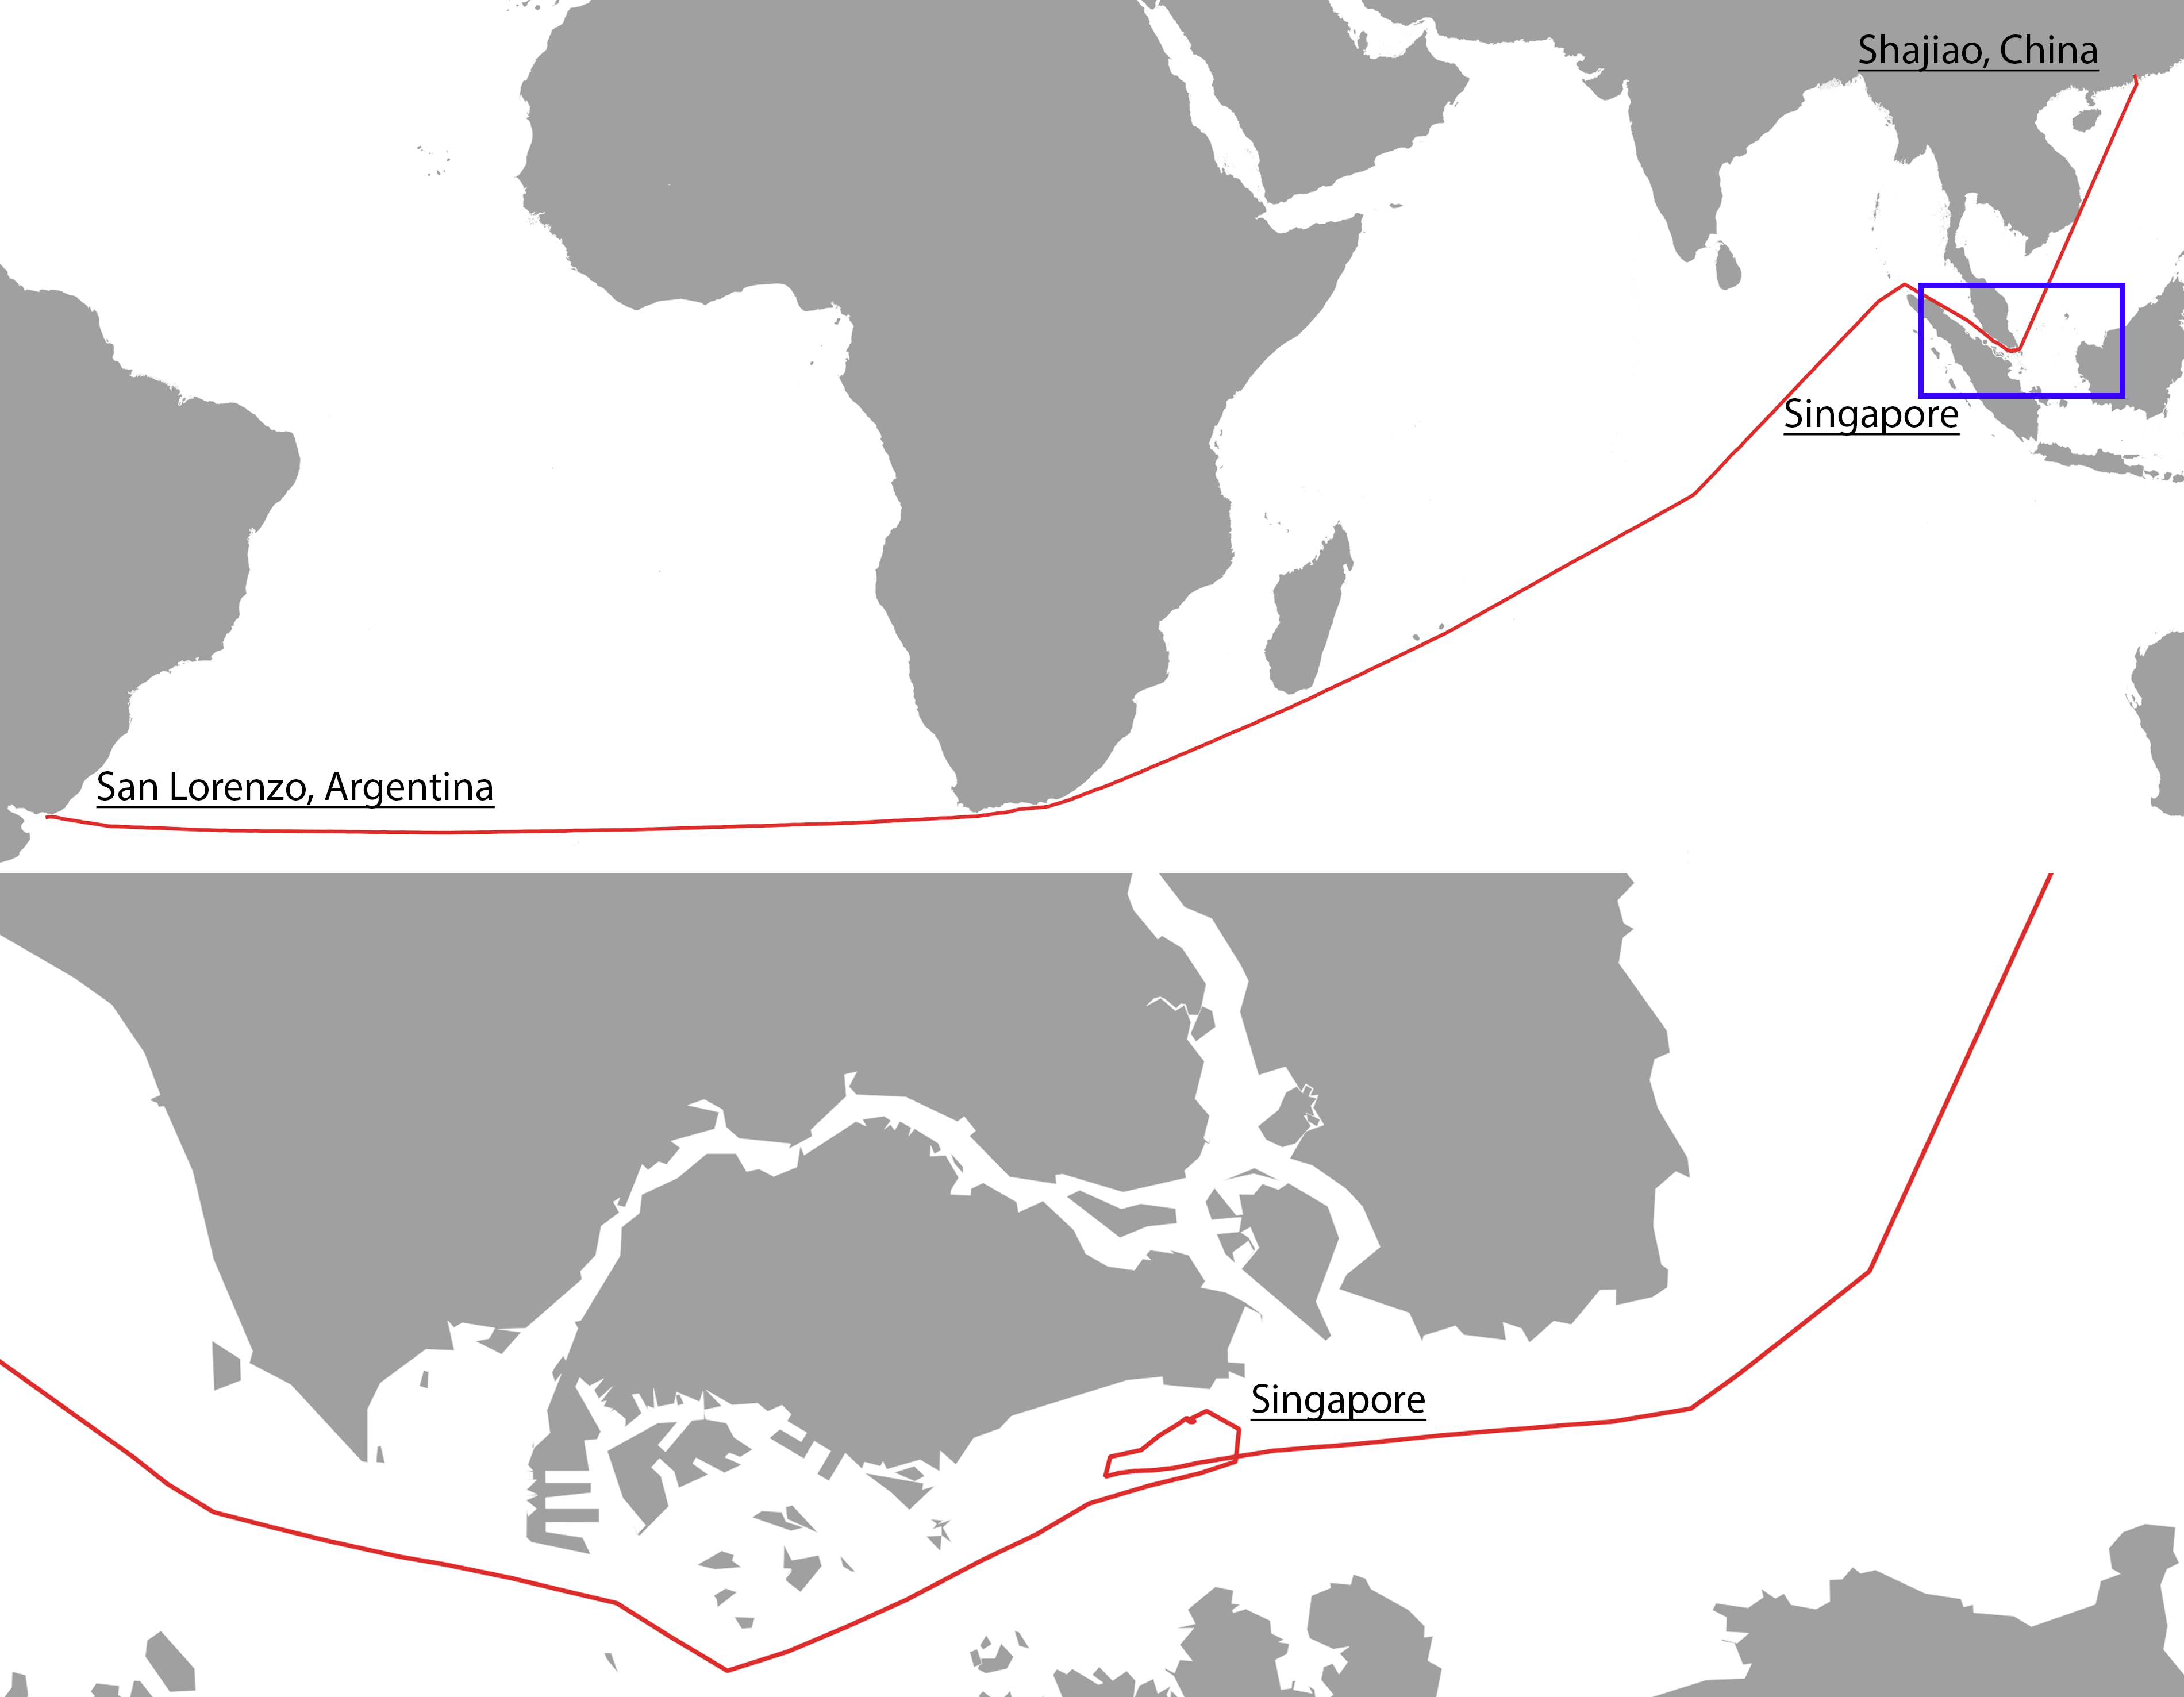
\includegraphics[width=1.0\textwidth]{figures/results/voyage_quality}
    \caption{Transition voyage from China to Argentina.}
    \label{fig:transition_voyage}
\end{figure}

The \textbf{1.7} million voyages constructed using the vessel transitions were sampled based on 6 hour intervals and collected in ``sampled\_transition\_voyages'' that formed the foundation for trajectory similarity measurements. In the process of constructing the final dataset, these sampled voyages were divided into multiple incomplete voyages up to a factor of four. The resulting training dataset collected in the table ``ml\_training\_data'' consisted of \textbf{4.3} million voyages.

\subsection{Trajectory similarity and MSTD}

Using the foundation of the sampled trajectories, each trajectory was compared to every other trajectory departing the same port to calculate the \acrfull{mstd}. The \acrshort{mstd} value was used primarily as a method of abstracting geographical trajectories into categorical and numerical values that a \acrfull{ml} model could work with. This process converted a voyage's geographical trajectory into MSTD, the similarity value to the most similar trajectory, and trajectory length. Thus, the MSTD value served as an initial prediction purely based on geographical trajectory similarity measurements using \acrfull{sspd}. The \acrshort{sspd} method was chosen for its ability to effectively handle different lengths and shapes of trajectories when estimating similarity. Furthermore, in the approach proposed in \cite{Zhang2020AISApproach} the \acrshort{sspd} method performed the best out of the algorithmic approaches evaluated, although, their own Random Forest (RF) based approach performed the best. However, the way the training data is structured, the trajectory similarity method of choice is completely interchangeable with others. The only requirement for a given trajectory similarity measurement is that it also produces a similarity value that serves as a weight for the \acrshort{mstd} value.

\acrshort{mstd} as an initial prediction seemed to be a decent initial indicator as to where the vessel would be arriving. In total, there were \textbf{4 306 271} entries in the final training data generated where exactly \textbf{1 423 476} of which has the same arrival port and \acrshort{mstd} value. Thus, it can be assumed that the purely spatial prediction using incomplete sampled historical voyages based on \acrshort{sspd} was \textit{33\%} accurate. In other words, when using an algorithmic prediction approach based on purely spatial trajectory similarity measurements, voyage destinations can be predicted correctly one third of the time. This formed a baseline accuracy to beat with the \acrshort{ml}-based solution.

\subsection{ML data preparation}

After the final training dataset was built, it was discovered that in terms of arrival port frequencies, the dataset was imbalanced thus making it harder for \acrshort{ml} models to learn. Although some models can better handle dataset imbalance, a sampling approach was used to balance the dataset before training to support different ML models. Several different sampling approaches were evaluated, however, the traditional over and under -sampling methods either produced massive amounts of synthetic data, or removed almost all the original data which was shown in \cref{fig:all_samplers} in \cref{chap:method}. Thus, an ensemble sampling method of majority undersampling and ``SMOTE+ENN'' was employed to balance the dataset before training. \cref{fig:ensemble_sampler} shows the results from the ensemble sampling method that uses a combination of under and over -sampling techniques. As \cref{fig:ensemble_sampler} shows, using a subset of the full dataset, the final result is 8\% smaller than the original dataset, is a lot more balanced, but still has differences in class frequencies which persisted from the original dataset.

\begin{figure}[htbp]
    \centering
    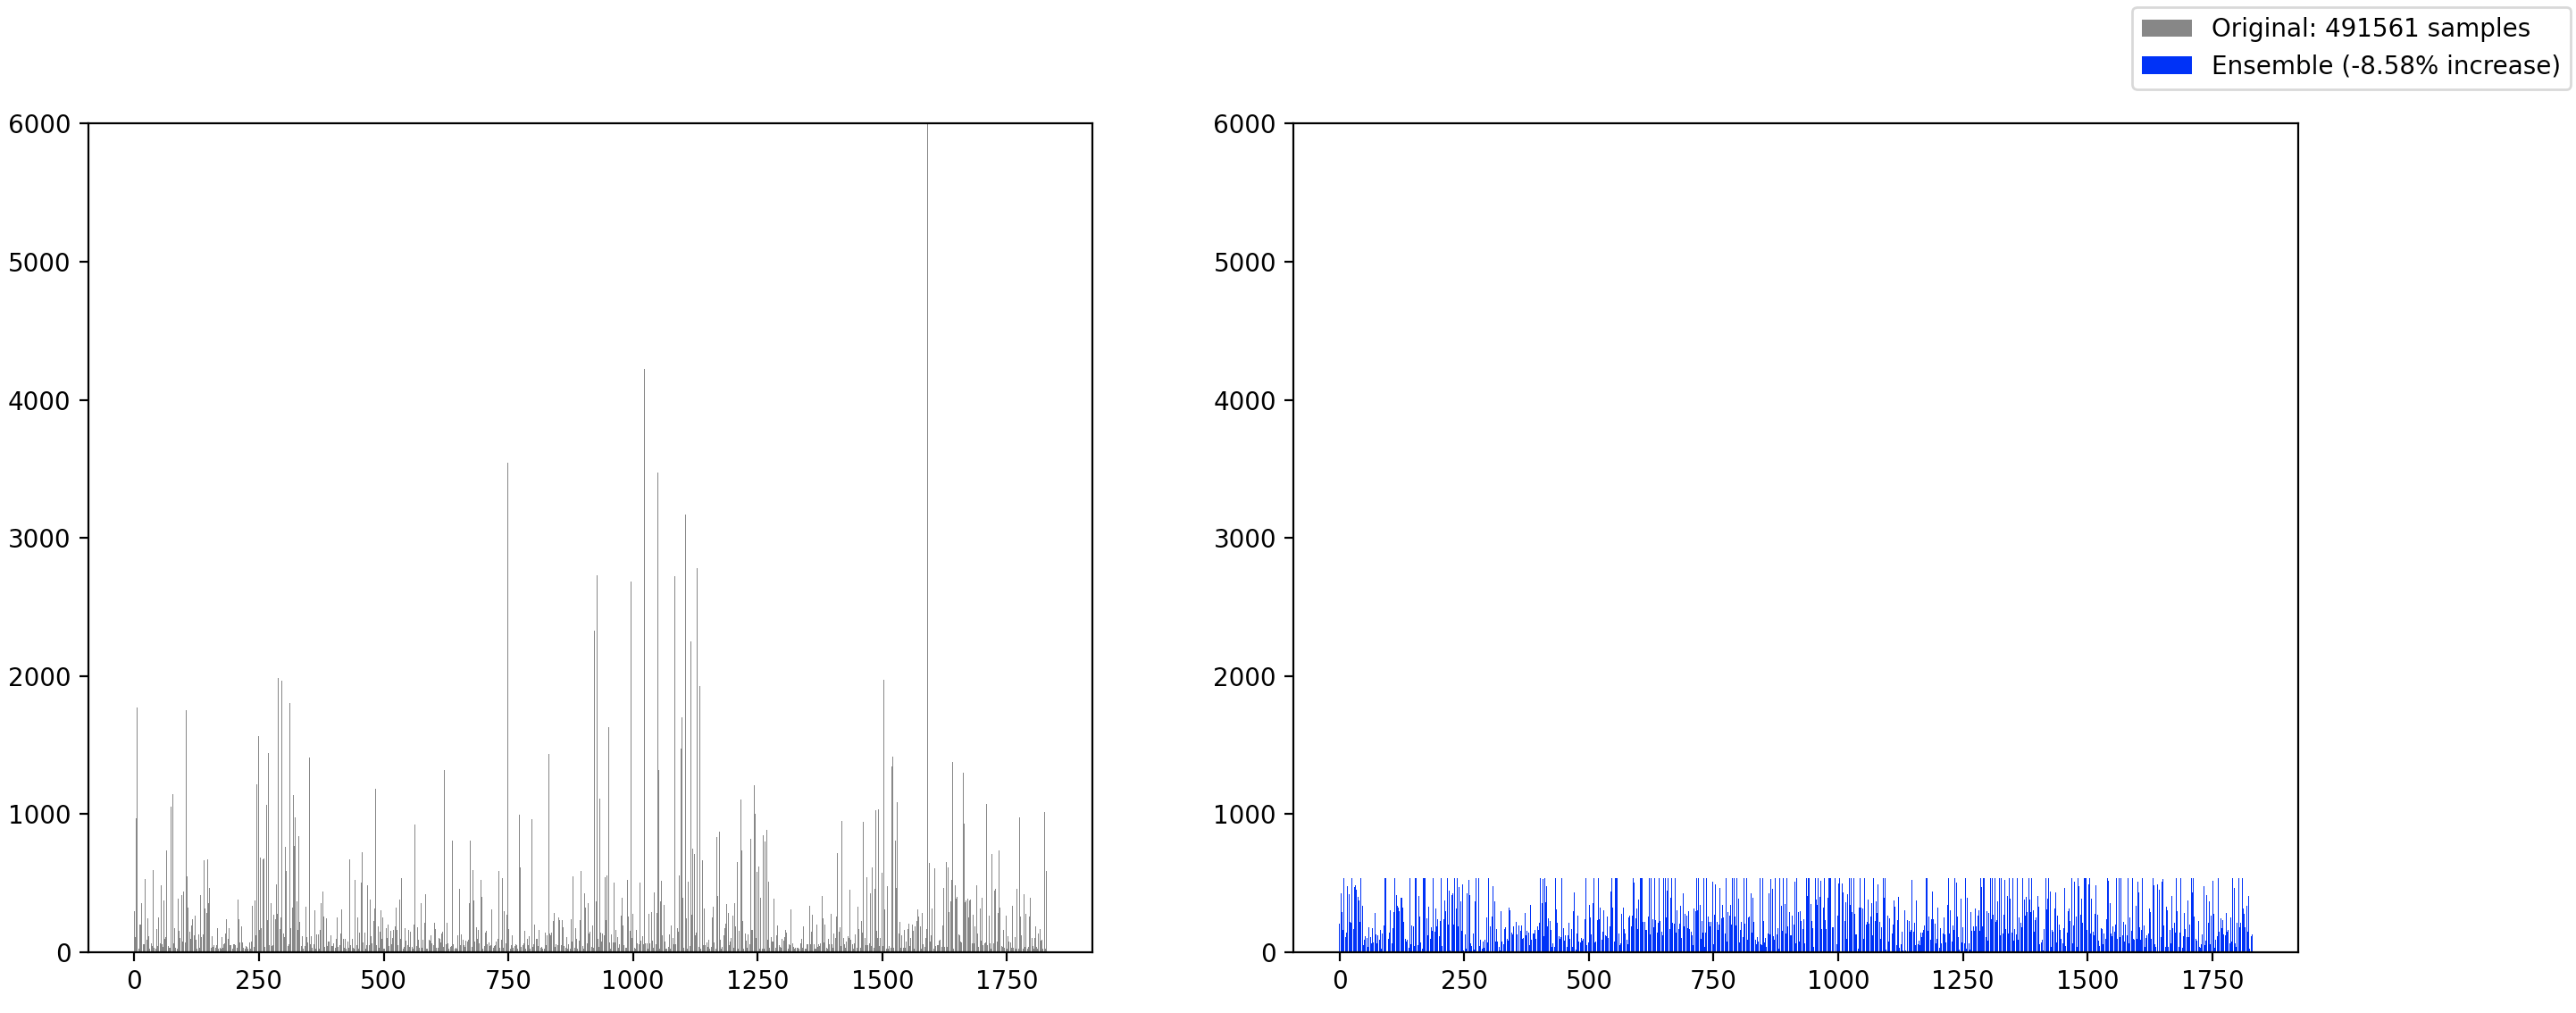
\includegraphics[width=1.0\textwidth]{figures/imbalance/ensemble}
    \caption{Final ensemble sampling method (right) compared to original dataset (left) where the final ensemble produces a dataset similar in size to that of the original.}
    \label{fig:ensemble_sampler}
\end{figure}

\section{Model training and prediction performance}

\subsection{Training process}

As described in \cref{sec:training_process}, multiple training processes were evaluated in order to find the most appropriate method of training a larger model on an extensive dataset. For the \acrfull{xgb} model, three different training processes were evaluated in this process.

First, the iterative approach was evaluated by training the model in batches of \textit{600 000} samples at the time. This approach seemed to work as intended, however, it was discovered that during subsequent training batches, the performance of the model dropped off for each iteration. It seemed as if the model did not handle continuous training of the same model as well as it does when training one model from scratch using the complete dataset. Furthermore, the parameter \textit{``early\_stopping\_rounds''} was used in the other approaches as a method of telling the model to stop training if it does not see any improvements after the given number of rounds. When this parameter is set using the iterative approach, the model can stop producing new trees before it has constructed the total number of trees allowed by the \textit{``n\_estimators''} parameter. Since the first iteration can produce a model with less trees than allowed, the next iteration fails as the number of allowed trees does not match with the previous model's actual number of trees. Although there are ways around this issue, as using the early stopping rounds parameter is useful to avoid overfitting, the iterative approach did not seem the most appropriate during the development process.

Next, it was attempted to train the model using the external memory, or ``out-of-core'' memory version of \acrshort{xgb}. In this approach, the \acrshort{xgb} library is provided a \textit{libsvm} file which it converts to an optimized matrix format which is kept on the computers file system. However, all attempts at training the model using external memory were unsuccessful as the training process consumed all of the running computer's available memory and resulted in a ``bad allocation`` memory error. There seems to either be a misconfiguration or an underlying issue with the Python library used in the implementation. However, since the expected results from this approach should be the same as training the model in one iteration on a capable computer, these issues were not further looked into, although, it could be beneficial to reduce the resource requirements for the training process for future use. Therefore, it could warrant more investigation for future work.

Finally, the entire dataset was used to train the final model in one iteration on a computer capable of running the process. The training process ran over the course of two days and consistently required around 200GB of memory. The vast memory consumption could be somewhat reduced by not evaluating the model during the training process which is appropriate for future training processes after the model has been trained and the training configuration has been validated. As described in \cref{sec:training_process}, an extra copy of the training and test datasets were kept in memory to continuously evaluate and monitor the training process.

\subsection{Performance}

\begin{figure}[htbp]
    \centering
    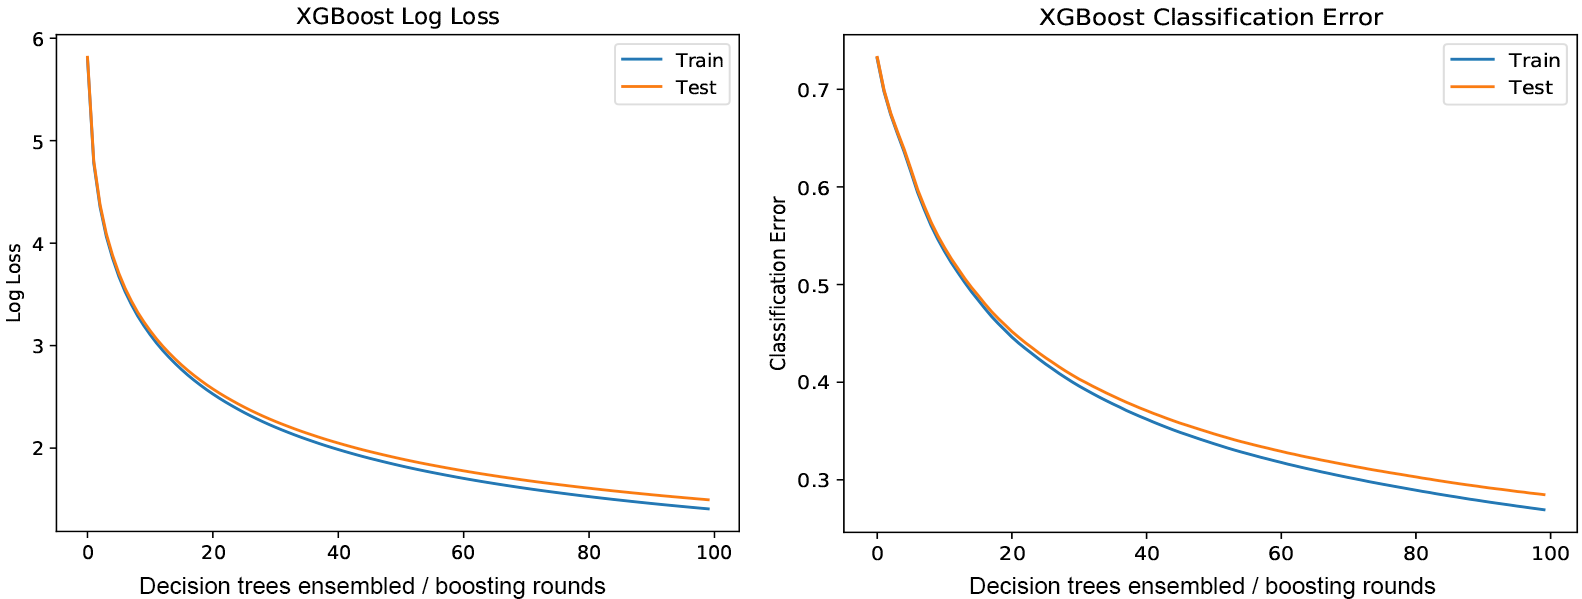
\includegraphics[width=1.0\textwidth]{figures/results/eval_set}
    \caption{Logarithmic loss and classification error metrics tracked per boosting round in the training process.}
    \label{fig:eval_set}
\end{figure}


\begin{lstlisting}[
    caption={Class report based on prediction results from the test dataset. The performance of the classifier is evaluated per class by using precition, recall, f1-score, support, and pred. \todo{update numbers}},
    label=lst:cv_result,
    showstringspaces=false,
    basicstyle=\ttfamily\medium,
]
[XGBoostClassifier] Class Report:
Class         precision    recall  f1-score  support    pred
1             0.545455  0.315789  0.400000     19.0    11.0
2             0.800000  1.000000  0.888889      4.0     5.0
3             0.666667  0.666667  0.666667      6.0     6.0
...           ...       ...       ...         ...     ...
253           0.333333  0.500000  0.400000      2.0     3.0
254           0.142857  0.500000  0.222222      2.0     7.0
255           0.833333  0.833333  0.833333      6.0     6.0
avg / total   0.657815  0.619792  0.621349   3072.0  3072.0
\end{lstlisting}


\begin{lstlisting}[
    caption={Output from 3-fold cross validation. \todo{update numbers}},
    label=lst:cv_result,
    showstringspaces=false,
    basicstyle=\ttfamily\medium,
]
 Folds:      [0.60569399 0.61297481 0.62244745]
 Mean:       0.6137054183485277
 Std. dev.:  0.006859056778768982
\end{lstlisting}

\section{Prediction results}

\subsection{Feature importances}

\begin{table}[htbp]
    \centering
    \begin{tabularx}{0.6\textwidth}{X X}
        \bfseries{Feature}  & \bfseries{Importance} \\ \toprule
        segmentation        & 0.314838 \\ \midrule
        sspd\_mstd          & 0.275234 \\ \midrule
        departure\_port     & 0.229567 \\ \midrule
        trajectory\_length  & 0.094224 \\ \midrule
        sspd\_dist          & 0.086137 \\ \bottomrule
    \end{tabularx}
    \caption{Feature importances based on the \acrshort{xgb} decision tree ensemble process. \todo{update numbers}}\label{tab:feature_importances}
\end{table}


\begin{itemize}
    \item Feature importances
    \item Impact of segment + sub-segment
    \item Impact of MSTD
\end{itemize}

\begin{lstlisting}[
    caption={Mean values of similarity value and trajectory length for correct and incorrect predictions.},
    label=lst:dist_length_impact,
    showstringspaces=false,
    tabsize=1,
    basicstyle=\ttfamily\medium,
]
mean sspd_dist for correct predictions:           100516.78046218488
mean trajectory_length for correct predictions:   14.785189075630251

mean sspd_dist for erroneous predictions:         108496.74400684932
mean trajectory_length for erroneous predictions: 15.434931506849315
\end{lstlisting}

\subsection{Segment predictability}

\begin{figure}[htbp]
    \centering
    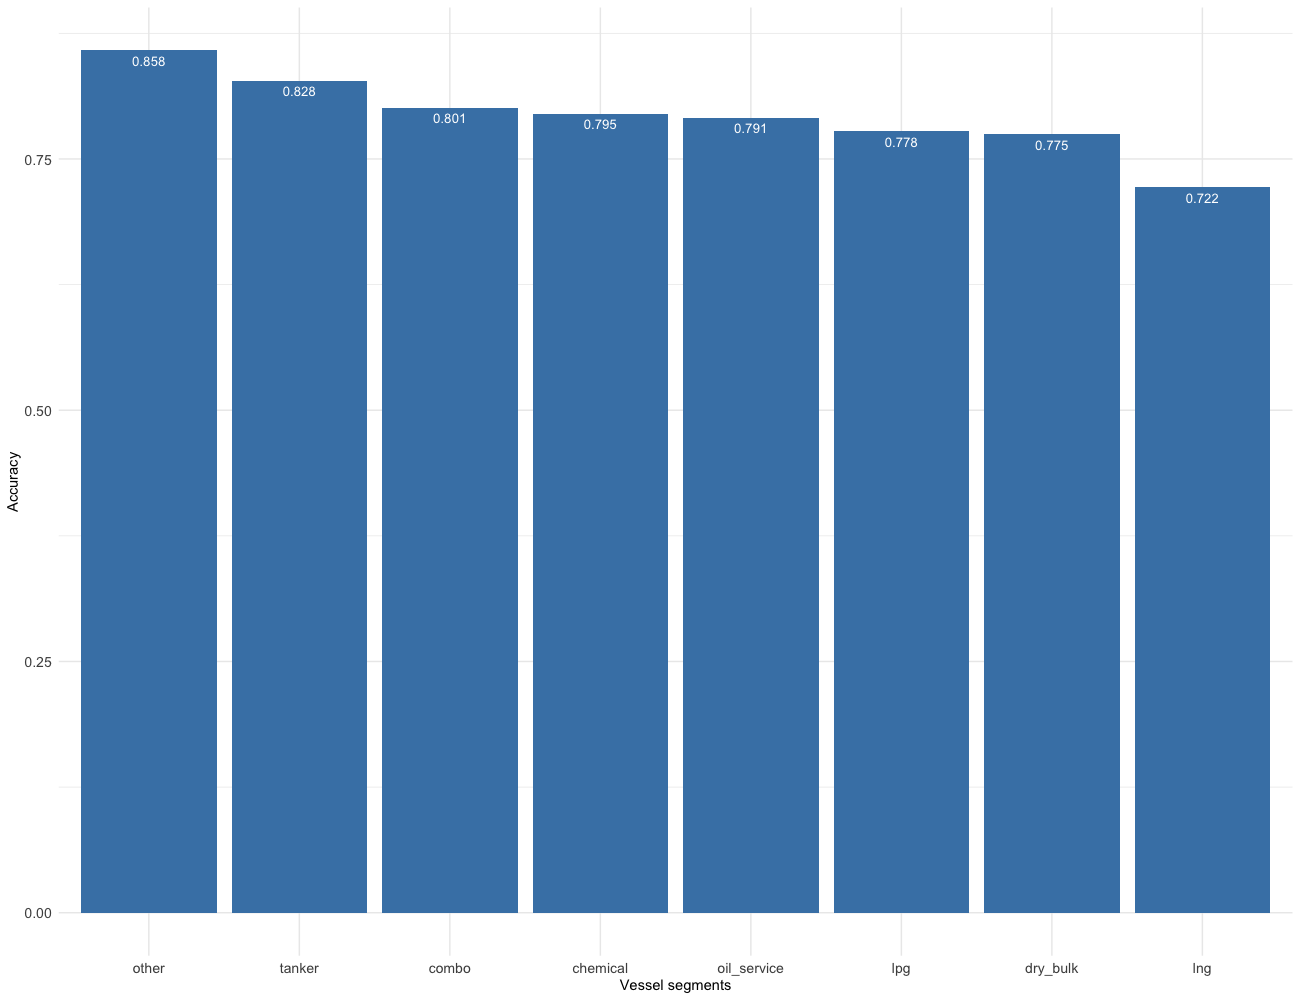
\includegraphics[width=1.0\textwidth]{figures/results/segment_accuracy}
    \caption{Accuracy of predictions from test set per segment.}
    \label{fig:segment_accuracy}
\end{figure}

\begin{itemize}
    \item What segments were easy to predict
    \item What sub-segments were easy to predict
\end{itemize}

\section{Real-life applications}

\subsection{Stand-alone usability}

\subsection{Integration with \acrfull{mo}}

\subsection{External evaluation from real shipping actors}

\begin{itemize}
    \item Caveats/use-cases and value
    \item Evaluation from MO
    \item Evaluation from external actors
\end{itemize}
